\documentclass[11pt]{article}
\usepackage[margin=1in]{geometry}
\usepackage[T1]{fontenc}
\usepackage{lmodern}
\usepackage{booktabs}
\usepackage{tikz}
\usetikzlibrary{arrows.meta,positioning}
\usepackage[numbers]{natbib}
\usepackage{hyperref}

\title{Does a Weekly Planning Prompt Improve Course Retention?\\A Field Study in an Online Statistics Course}
\author{Dana Whitfield and Marcus Oyelaran\\Department of Information Systems, Westbrook State University}
\date{}

\begin{document}
\maketitle

\begin{abstract}
Online courses lose many students in the first month. We tested whether a short weekly planning prompt, delivered inside the course site, raises retention to week eight. In a field study of 612 students across two terms, students who received the prompt were more likely to remain enrolled and to submit the midterm. The effect held in both terms. However, it was smaller for students who had already logged in at least four times in week one.
\end{abstract}

\section{Introduction}
Attrition in online courses is common and costly \citep{davis1989}. Students who leave early rarely return, and instructors often learn about the problem only after the first graded assignment. Interventions that act before that point are therefore valuable, provided they are cheap enough to run in every section.

Planning prompts are one such intervention. A prompt asks a student to name when and where they will complete the coming week's work. Prior studies of planning prompts report gains in task completion, but most were run in laboratory settings or in a single course. It remains unclear whether a prompt delivered through a learning management system changes retention over several weeks.

This study addresses that gap. We ask two questions. First, does a weekly planning prompt raise retention to week eight? Second, does the effect depend on how engaged a student is at the start of the course?

\section{Method}
We recruited 612 students from 14 sections of an introductory statistics course taught online over two consecutive terms. Sections were randomly assigned to a prompt condition or a control condition. Students in the prompt condition saw a two-question form each Monday asking when they planned to study and which task they would start first. Control students saw the usual weekly announcement.

We measured retention as remaining enrolled at the end of week eight. We also recorded whether the student submitted the midterm, and the number of logins in week one. Analyses used logistic regression with term as a covariate, and we report odds ratios with 95\% confidence intervals.

\section{Results}
Retention to week eight was higher in the prompt condition than in the control condition. Table~\ref{tab:retention} summarises the outcomes by condition. The the difference in midterm submission was similar in size to the difference in retention.

\begin{table}[t]
\centering
\caption{Retention and midterm submission by condition (N = 612).}
\label{tab:retention}
\begin{tabular}{lrrr}
\toprule
Condition & Students & Retained to week 8 & Submitted midterm \\
\midrule
Control & 305 & 71.8\% & 66.9\% \\
Planning prompt & 307 & 79.1\% & 74.6\% \\
\bottomrule
\end{tabular}
\end{table}

The odds of remaining enrolled were 1.50 times higher with the prompt (95\% CI [1.05, 2.15], $p = .027$). Figure~\ref{fig:model} shows the path we propose: the prompt increases early planning, which increases early engagement, which in turn supports retention. The effect was smaller for students with four or more logins in week one, which suggests that the prompt helps most where engagement is not already high.

\begin{figure}[t]
\centering
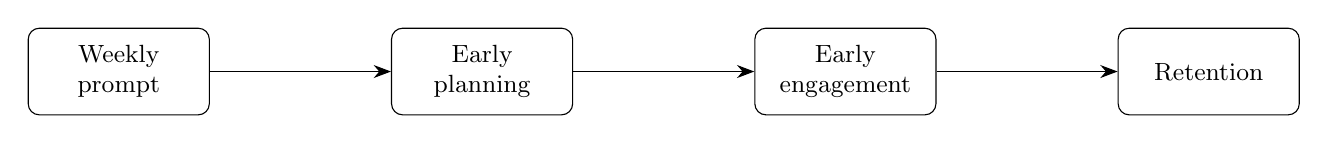
\begin{tikzpicture}[node distance=2.3cm, every node/.style={draw, rounded corners, align=center, minimum height=1.1cm, minimum width=2.3cm, font=\small}, >={Stealth[length=2.2mm]}]
\node (a) {Weekly\\prompt};
\node (b) [right=of a] {Early\\planning};
\node (c) [right=of b] {Early\\engagement};
\node (d) [right=of c] {Retention};
\draw[->] (a) -- (b);
\draw[->] (b) -- (c);
\draw[->] (c) -- (d);
\end{tikzpicture}
\caption{The proposed path from the weekly planning prompt to retention.}
\label{fig:model}
\end{figure}

\section{Discussion}
A weekly planning prompt raised retention by about seven percentage points in this sample. The prompt takes one minute to answer, requires no instructor time, and can be added to any course site. These properties make it a plausible default for large introductory courses.

The study has three limitations. First, sections rather than students were randomised, so section-level differences may account for part of the effect. Second, retention was measured only to week eight. Third, we did not observe whether students followed the plans they wrote. Future work should randomise individual students and extend follow-up to the end of the term.

\bibliographystyle{plainnat}
\bibliography{refs}
\end{document}
